\documentclass{beamer}

\mode<presentation> {
    \usetheme{} 
    \setbeamertemplate{footline}[page number] 
    \setbeamertemplate{navigation symbols}{} 
    \setbeamertemplate{caption}[numbered]
}

\title{\textbf{Lotka-Volterra equations}}

\author{Amin, Paddy, Kam, Yasir, Sam}

\begin{document}
    \titlepage
    
    \begin{frame}{VSCode \& Linux/Unix}
        \begin{figure}
            \centering
            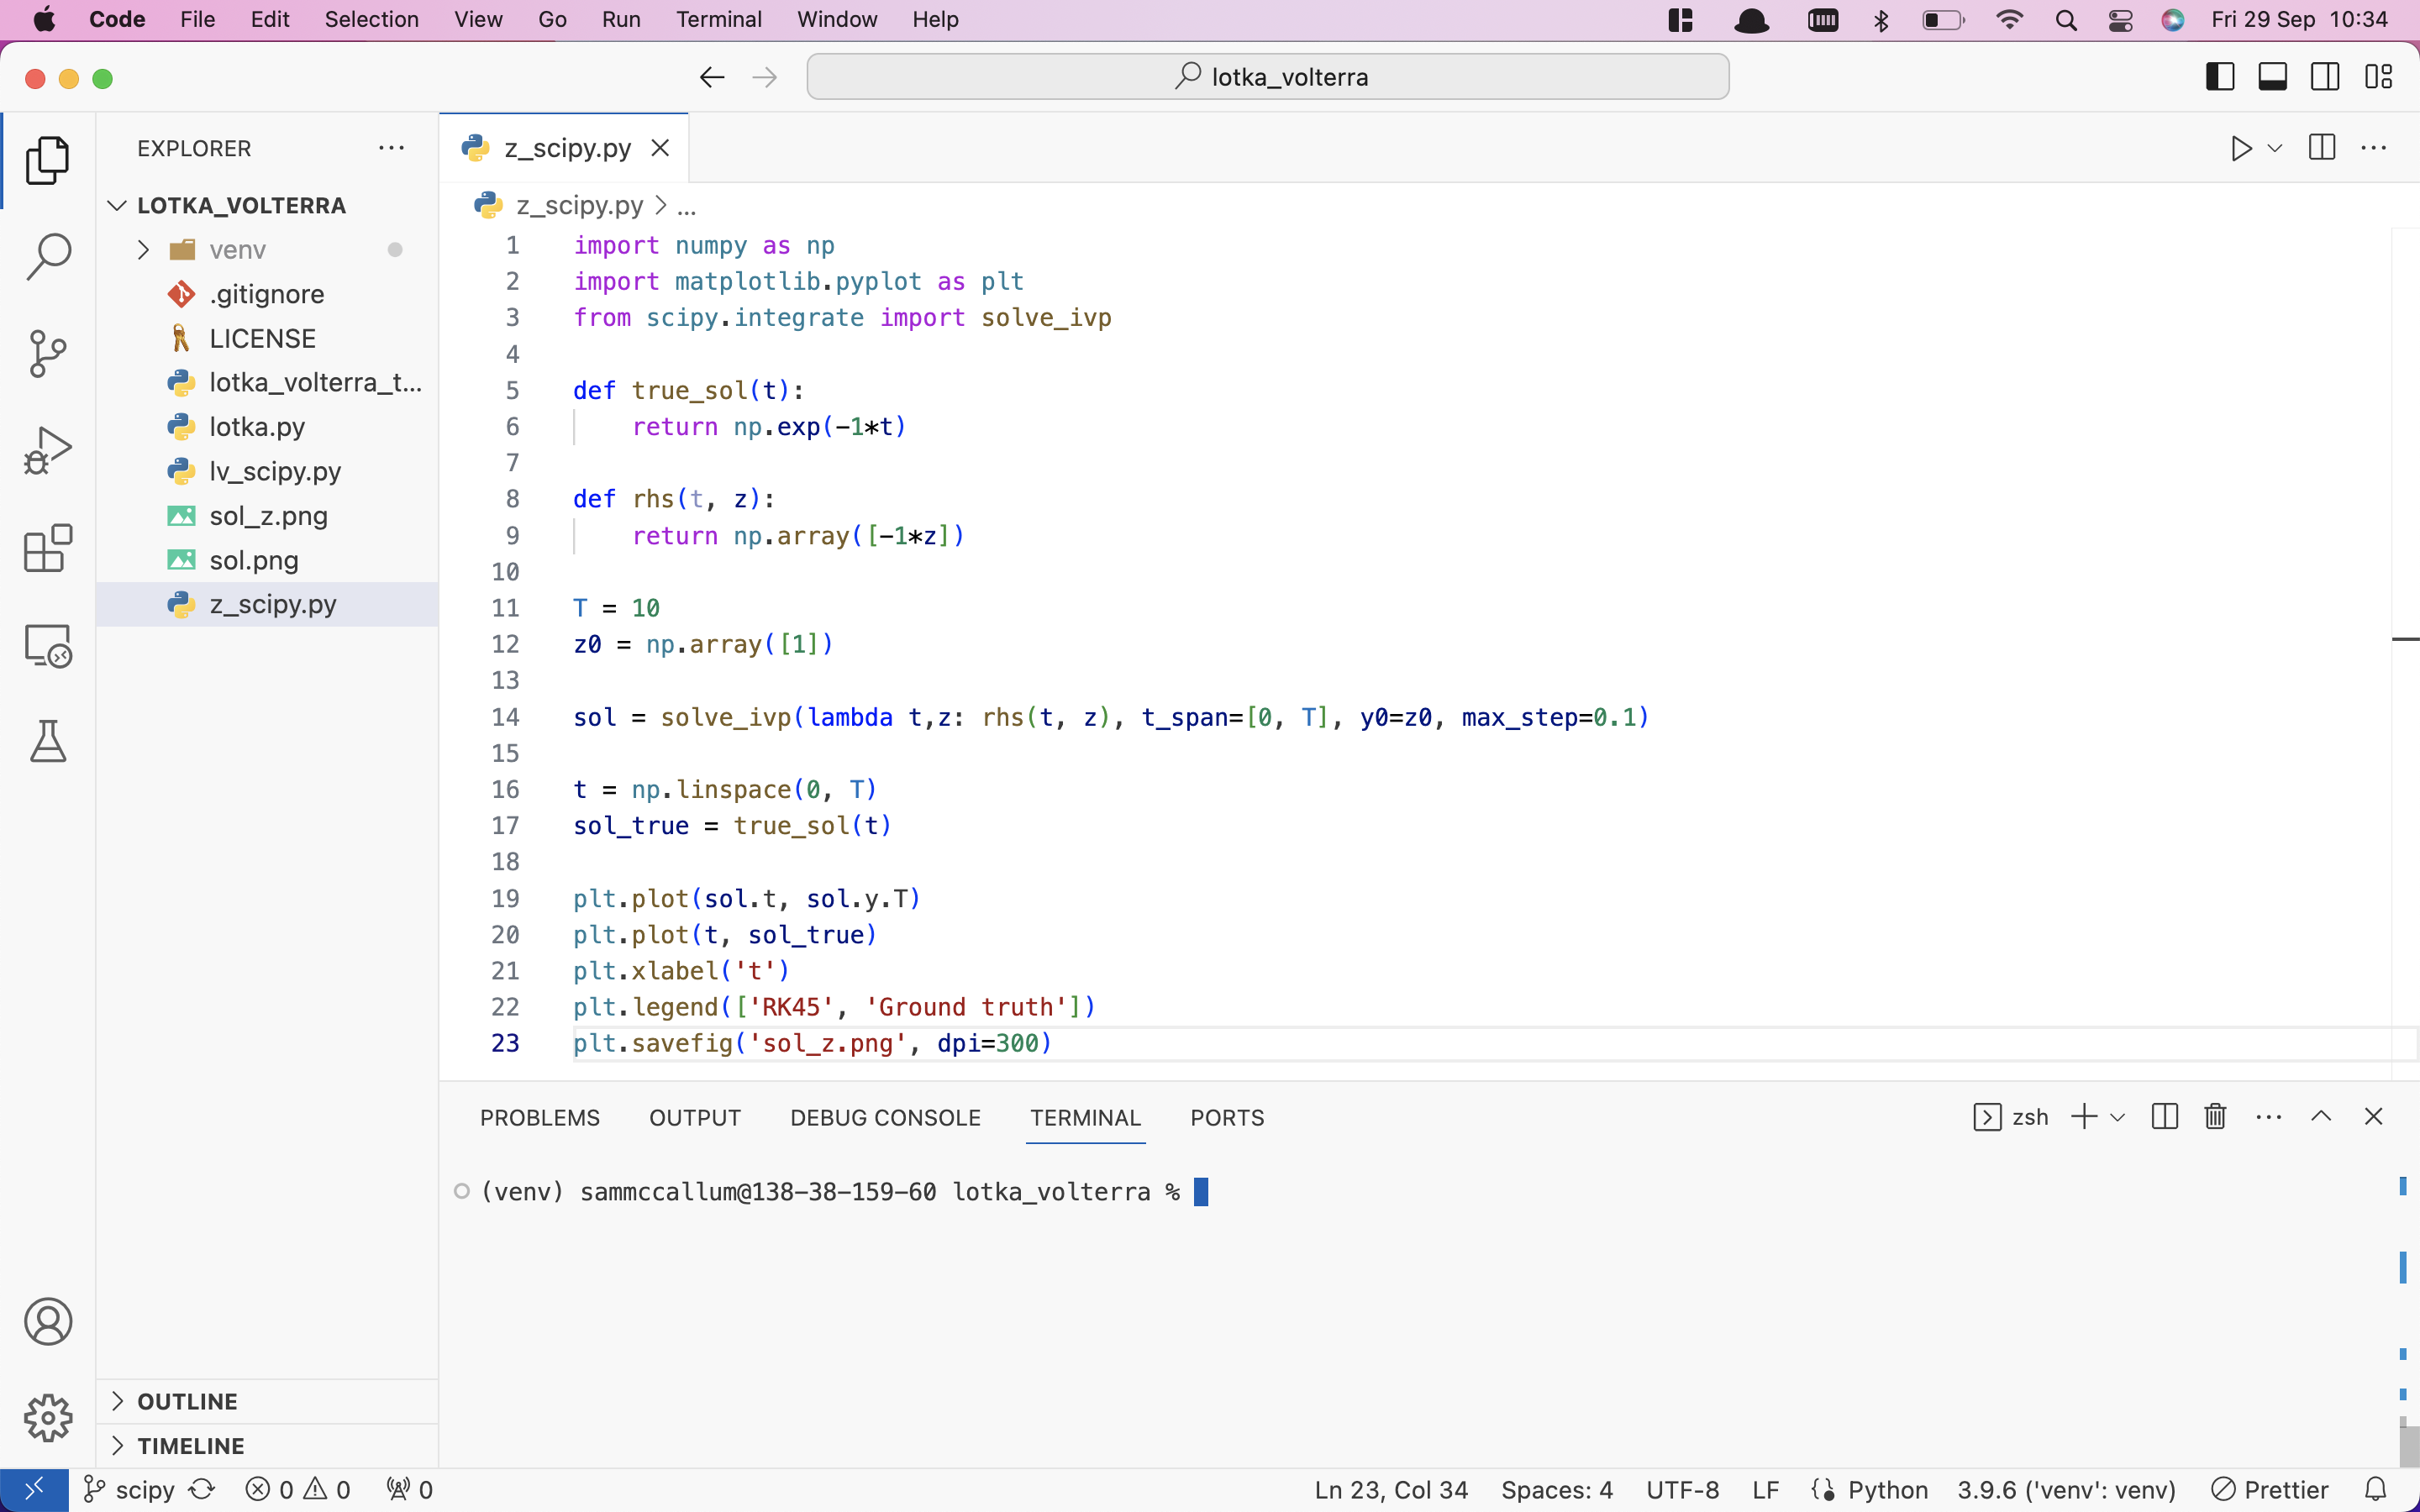
\includegraphics[width=\textwidth]{vscode.png}
            \label{fig:vscode}
        \end{figure}
    \end{frame}

    \begin{frame}{Git \& GitHub}
        \begin{figure}
            \centering
            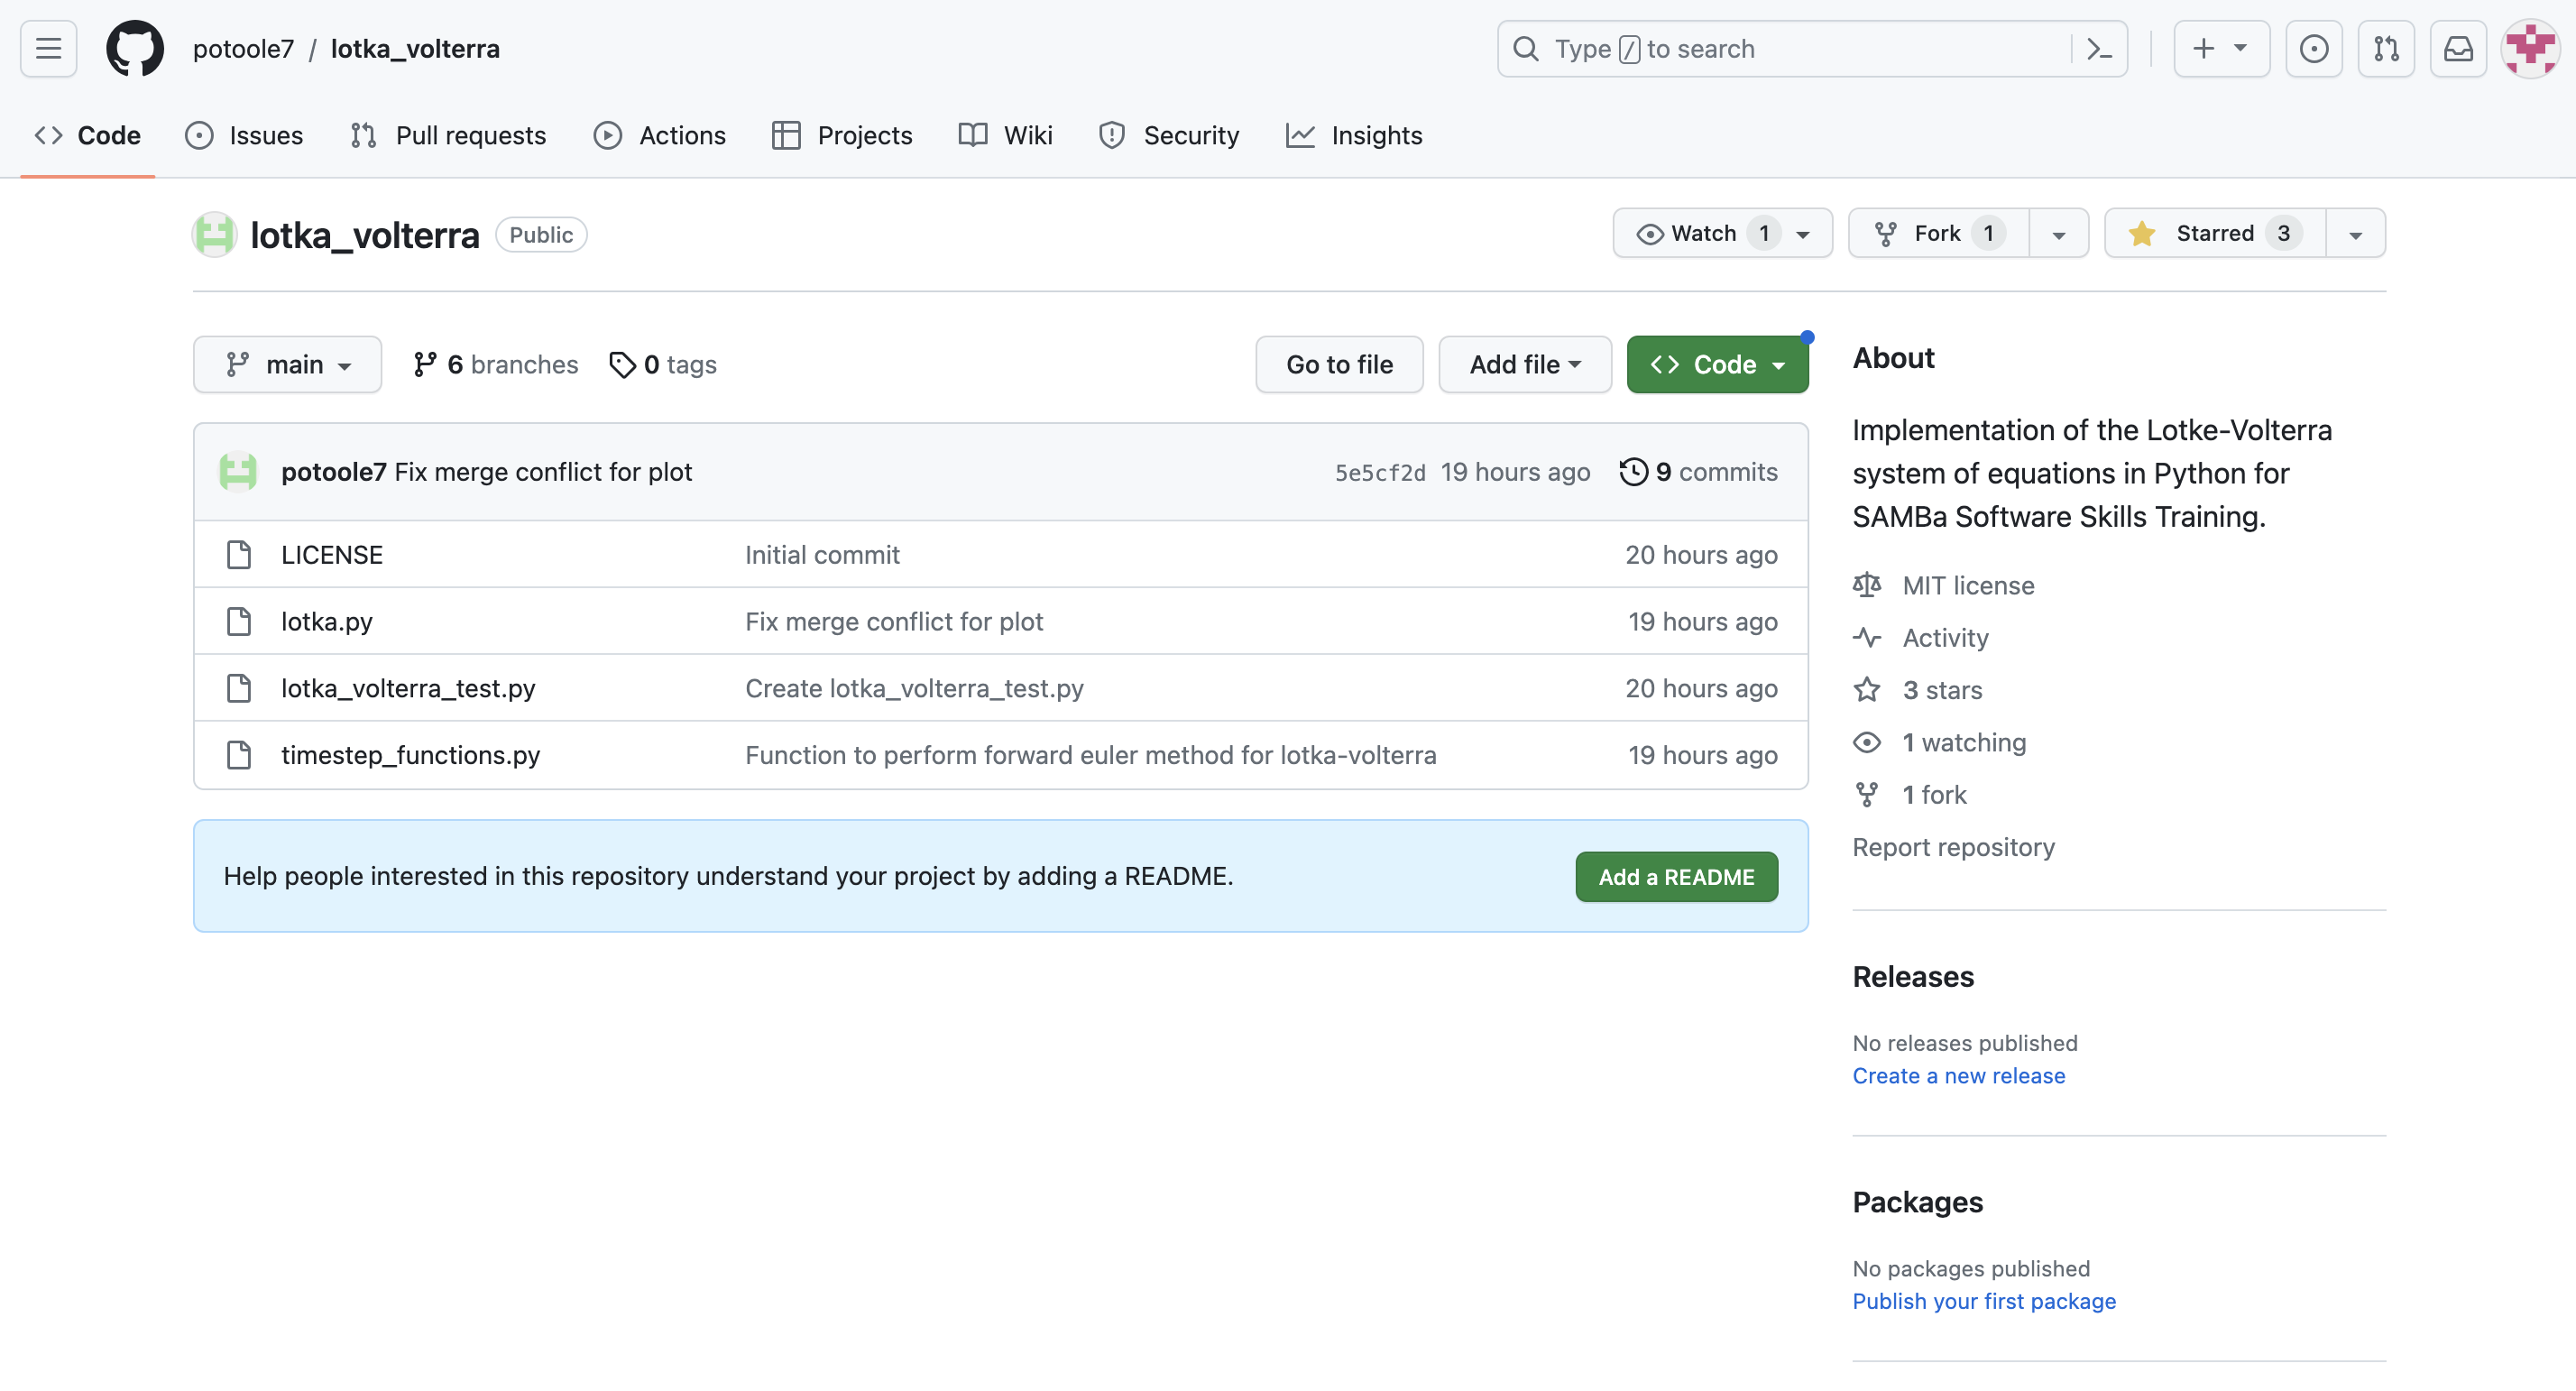
\includegraphics[width=\textwidth]{github.png}
            \label{fig:github}
        \end{figure}
    \end{frame}

    \begin{frame}{Scientific libraries}
        \begin{figure}
            \centering
            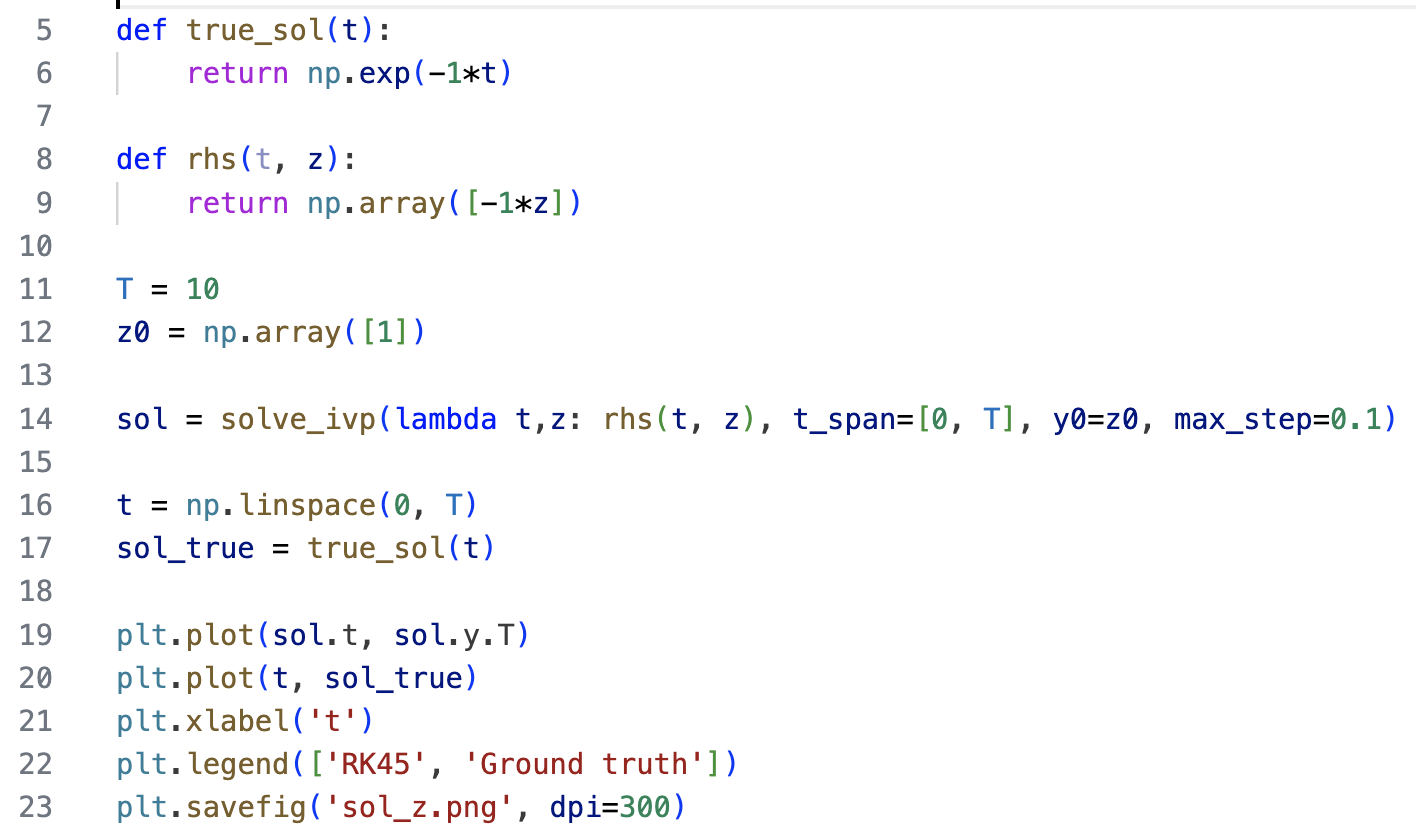
\includegraphics[width=\textwidth]{scientific-libraries.png}
            \label{fig:scilib}
        \end{figure}
    \end{frame}
    
\end{document}
